% !Mode:: "TeX:EN:UTF-8:Main"
%created with by @marmot 14.09.2018
%
\documentclass[border=3.14mm,tikz]{standalone}
\usetikzlibrary{fit,matrix,positioning,arrows.meta,decorations.text,shapes.callouts}
\pgfdeclarelayer{background}
\pgfdeclarelayer{container}
\pgfdeclarelayer{foreground}
\pgfsetlayers{container,background,main,foreground}
\usepackage {fontspec}
\usepackage {unicode-math}
\usepackage{tikzmarmots,tikzducks}

\setmainfont[
% Numbers     = OldStyle, %% buggy with font cache
  Ligatures   = TeX,
  BoldFont    = {Linux Libertine O Bold},
  ItalicFont  = {Linux Libertine O Italic},
  SlantedFont = {Linux Libertine O Italic},
]{Linux Libertine O}
\setmonofont[Ligatures=TeX,Scale=MatchLowercase]{Liberation Mono}
%setsansfont[Ligatures=TeX]{Linux Biolinum O}
\setsansfont[Ligatures=TeX,Scale=MatchLowercase]{Iwona Medium}
\begin{document}
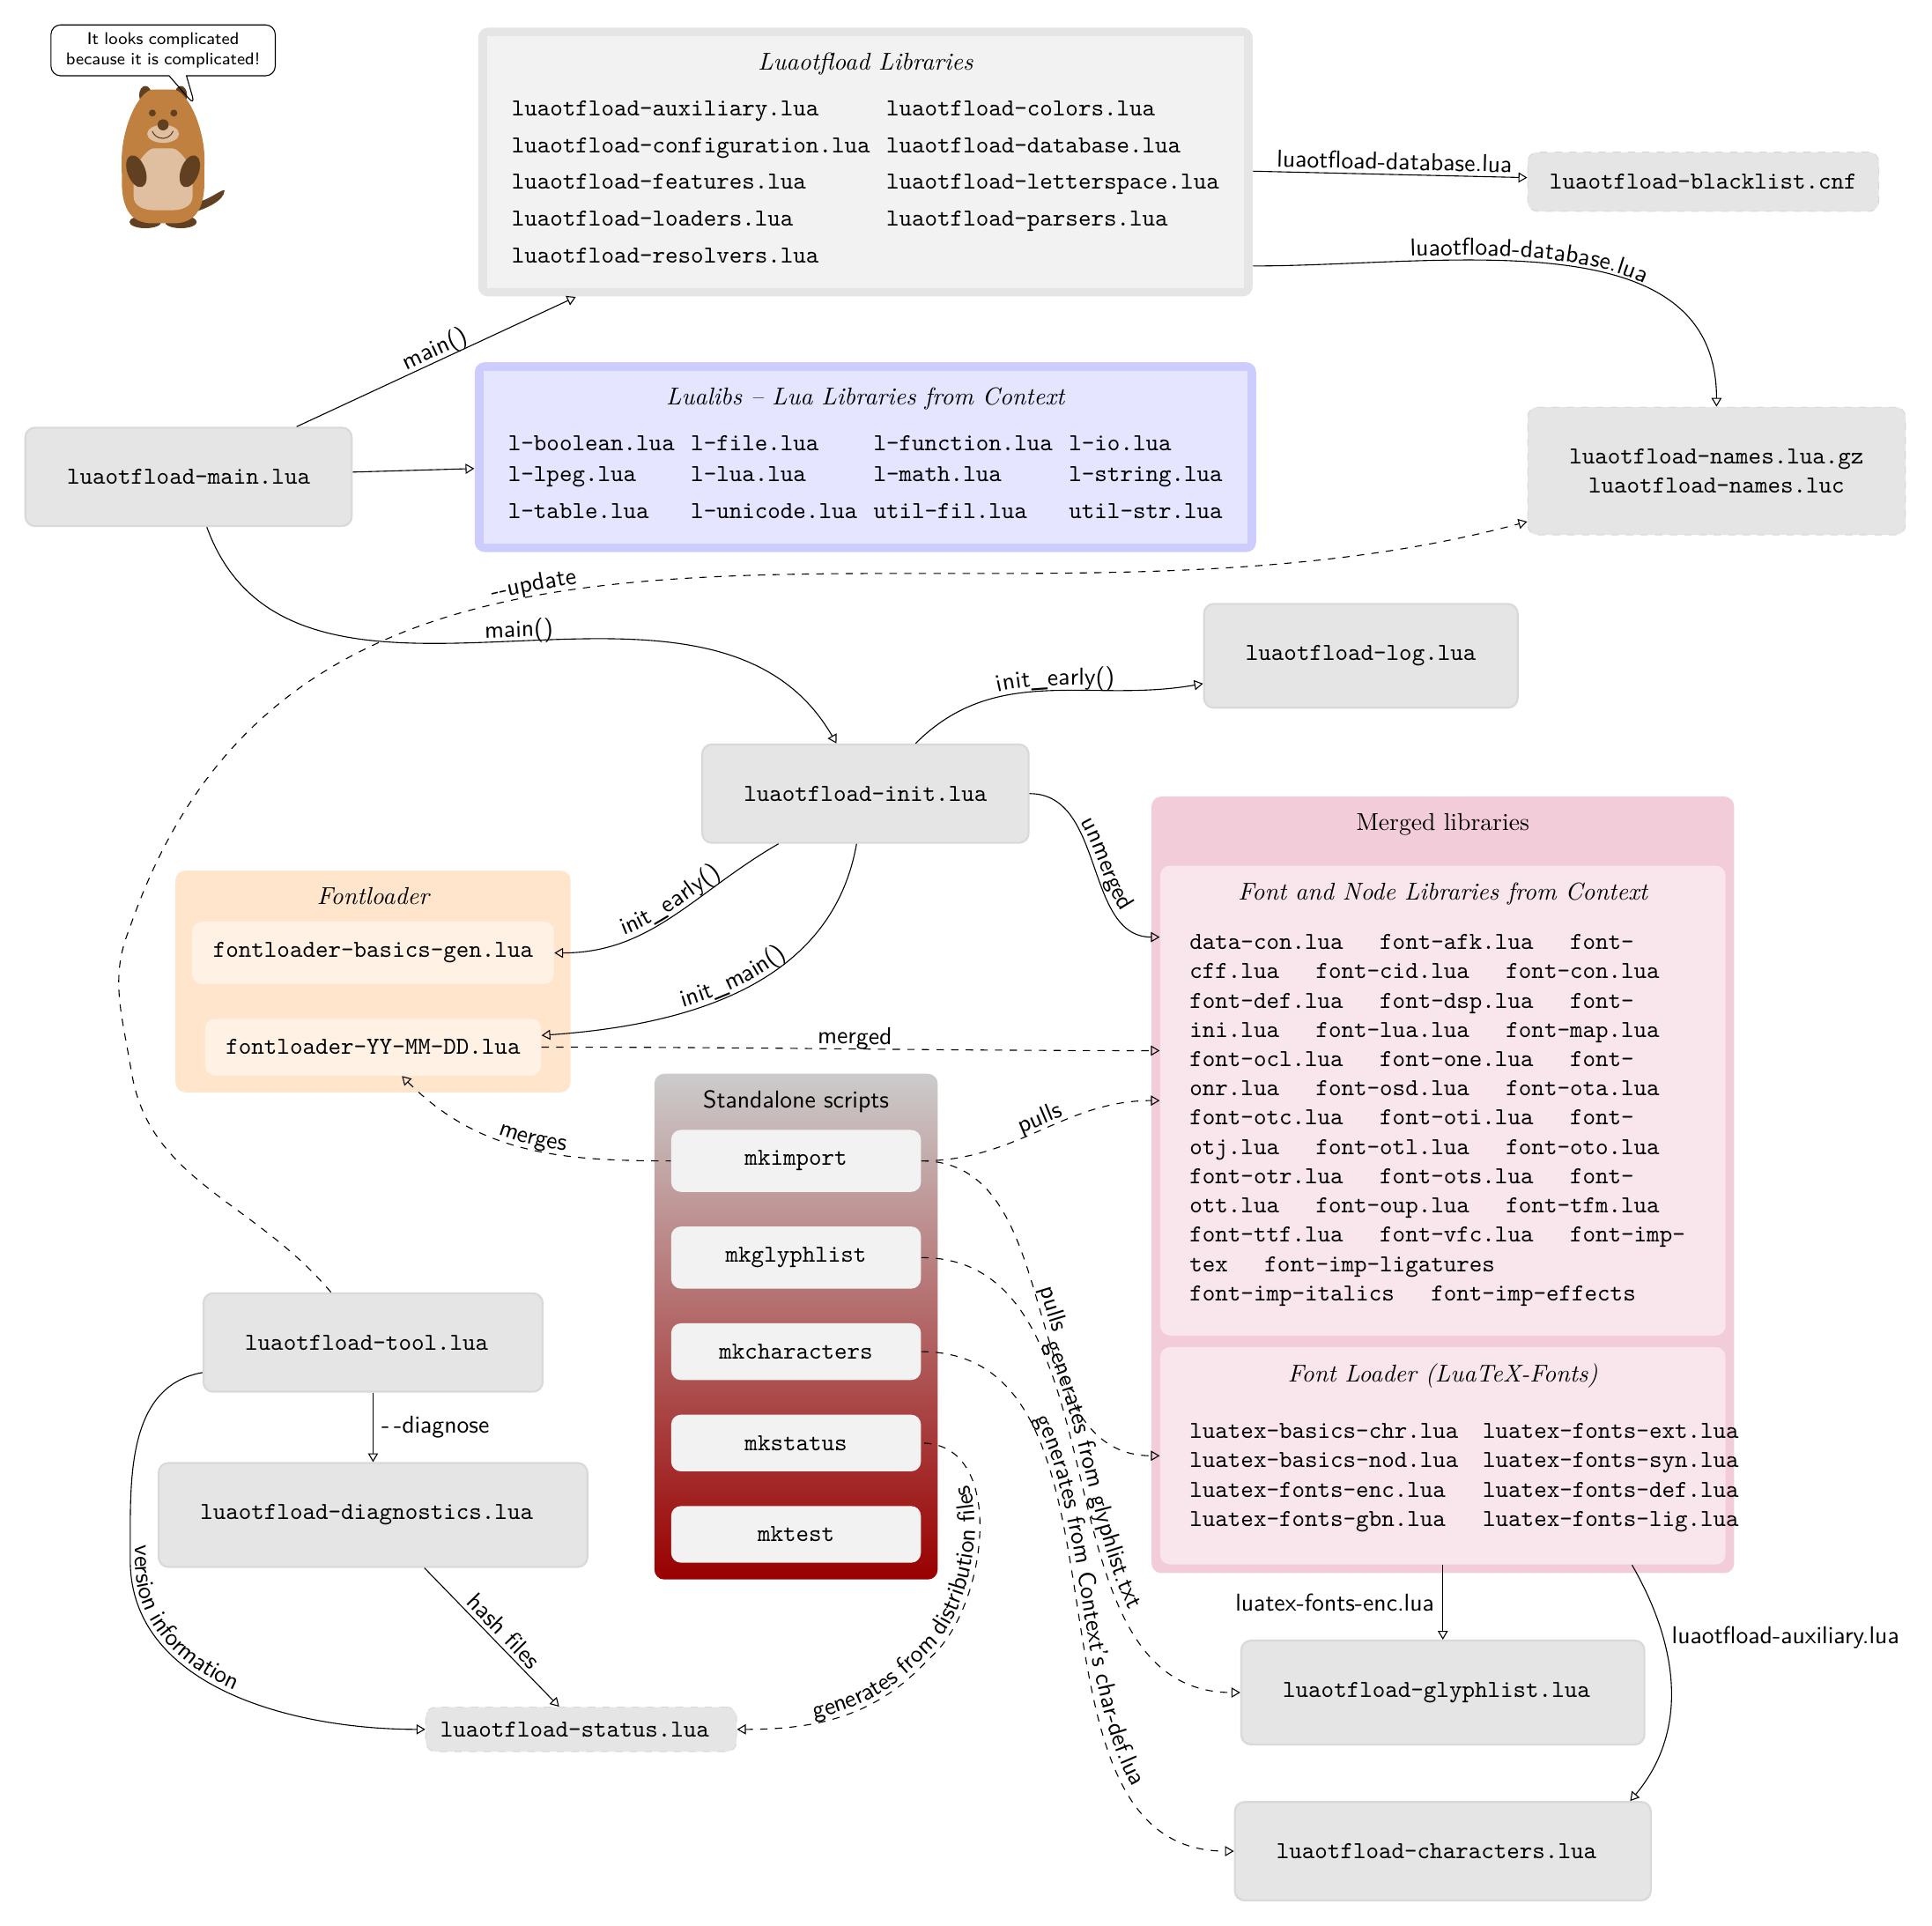
\begin{tikzpicture}[rounded corners,basic/.style={inner
sep=9pt,font=\ttfamily,align=center}]
%%%%%%%%%%%%%%%%%%%%%%%%%%%%%%%%%%%%%%%%%%
% text nodes
%%%%%%%%%%%%%%%%%%%%%%%%%%%%%%%%%%%%%%%%%%
% m1
\matrix [matrix of nodes,font=\ttfamily,nodes={anchor=base west},
label={[name=mL1,font=\itshape]above:Luaotfload Libraries}] (m1)
{%
%<<<<<<<<<<<<<<<<
luaotfload-auxiliary.lua    &
luaotfload-colors.lua       \\
luaotfload-configuration.lua &
luaotfload-database.lua     \\
luaotfload-features.lua     &
luaotfload-letterspace.lua  \\
luaotfload-loaders.lua      &
luaotfload-parsers.lua      \\
luaotfload-resolvers.lua    \\
%>>>>>>>>>>>>>>>>
};
% m2	
\node[right=4.2cm of m1,fill=gray!20,draw=gray!30,dashed,basic] (m2) {luaotfload-blacklist.cnf};	
% m3
\matrix [below=2cm of m1,matrix of nodes,font=\ttfamily,nodes={anchor=base west},
label={[name=mL3,font=\itshape,anchor=south]above:Lualibs -- Lua Libraries from Context}] (m3)
{%
%<<<<<<<<<<<<<<<<
l-boolean.lua &
l-file.lua &
l-function.lua&
l-io.lua \\
l-lpeg.lua &
l-lua.lua &
l-math.lua &
l-string.lua \\
l-table.lua &
l-unicode.lua &
util-fil.lua&
util-str.lua\\
%>>>>>>>>>>>>>>>>
};
% m4	
\node[left=2cm of m3,fill=gray!20,draw=gray!30,thick,basic,inner sep=6mm] (m4) {luaotfload-main.lua};	
% m5
\node[fill=gray!20,draw=gray!30,dashed,basic,inner sep=6mm,anchor=south west] at (m3.south -|
m2.west)(m5){%
%<<<<<<<<<<<<<<<<
luaotfload-names.lua.gz\\ 
luaotfload-names.luc
%>>>>>>>>>>>>>>>>
};	
% m6
\node[below=3cm of m3,fill=gray!20,draw=gray!30,thick,basic,inner sep=6mm] (m6){luaotfload-init.lua};	
% m7
\node[above right=0.5cm and 2.5cm of m6,fill=gray!20,draw=gray!30,thick,basic,inner sep=6mm] (m7){luaotfload-log.lua};	
% m8
\matrix [below left=1cm and 2cm of m6,matrix of nodes,font=\ttfamily,
row sep=5mm,
nodes={inner sep=3mm,fill=orange!10,rounded corners},
label={[name=mL8,font=\it]above:Fontloader}] (m8)
{%
%<<<<<<<<<<<<<<<<
fontloader-basics-gen.lua\\
fontloader-YY-MM-DD.lua\\
%<<<<<<<<<<<<<<<<
};
% m9
\node [below right=1cm and 2cm of m6,font=\ttfamily,
inner sep=3mm,text width=7.3cm,align=left,
label={[name=mL9,font=\itshape]Font and Node Libraries from Context}] (m9)
{\spaceskip=1.5em
%%<<<<<<<<<<<<<<<<
data-con.lua
font-afk.lua
font-cff.lua
font-cid.lua
font-con.lua
font-def.lua
font-dsp.lua
font-ini.lua
font-lua.lua
font-map.lua
font-ocl.lua
font-one.lua
font-onr.lua
font-osd.lua
font-ota.lua
font-otc.lua
font-oti.lua
font-otj.lua
font-otl.lua
font-oto.lua
font-otr.lua
font-ots.lua
font-ott.lua
font-oup.lua
font-tfm.lua
font-ttf.lua
font-vfc.lua
font-imp-tex
font-imp-ligatures\\
font-imp-italics
font-imp-effects
%>>>>>>>>>>>>>>>>
};
% m10
\node [below=1cm of m9,font=\ttfamily,
inner sep=3mm,text width=7.3cm,align=center,
label={[name=mL10,font=\itshape]Font Loader (LuaTeX-Fonts)}] (m10)
{\tabcolsep=0.5em
 \begin{tabular}{@{}ll@{}}
%<<<<<<<<<<<<<<<<
luatex-basics-chr.lua   & 
luatex-fonts-ext.lua   \\
luatex-basics-nod.lua   & 
luatex-fonts-syn.lua   \\
luatex-fonts-enc.lua    & 
luatex-fonts-def.lua   \\
luatex-fonts-gbn.lua    &
luatex-fonts-lig.lua
%>>>>>>>>>>>>>>>> 
 \end{tabular}
};
% m11
\node [above=1cm of m9] (m11) {Merged libraries};
% m12
\matrix [below=4cm of m6,xshift=-1cm,matrix of nodes,font=\ttfamily,
row sep=5mm,
nodes={inner sep=3mm,fill=gray!10,rounded corners,text width=3cm,align=center},
label={[name=mL12,font=\sffamily]above:Standalone scripts}] (m12)
{%
%<<<<<<<<<<<<<<<<
mkimport\\
mkglyphlist\\
mkcharacters\\
mkstatus\\
mktest\\
%>>>>>>>>>>>>>>>> 
};
% m13
\node[below=1.2cm of m10,fill=gray!20,draw=gray!30,thick,basic,inner sep=6mm]	(m13) 
{%
%<<<<<<<<<<<<<<<<
luaotfload-glyphlist.lua
%>>>>>>>>>>>>>>>> 
};
% m14
\node[below=0.8cm of m13,fill=gray!20,draw=gray!30,thick,basic,inner sep=6mm]	(m14) 
{%
%<<<<<<<<<<<<<<<<
luaotfload-characters.lua
%>>>>>>>>>>>>>>>> 
};
% m15
\node[below=3cm of m8,fill=gray!20,draw=gray!30,thick,basic,inner sep=6mm]	
(m15) {%
%<<<<<<<<<<<<<<<<
luaotfload-tool.lua
%>>>>>>>>>>>>>>>> 
};
% m16
\node[below=1cm of m15,fill=gray!20,draw=gray!30,thick,basic,inner sep=6mm]	
(m16) {%
%<<<<<<<<<<<<<<<<
luaotfload-diagnostics.lua
%>>>>>>>>>>>>>>>> 
};
% m17
\node[below=2cm of m16,xshift=3cm,fill=gray!20,draw=gray!30,dashed,basic,inner sep=6pt]	
(m17) {%
%<<<<<<<<<<<<<<<<
luaotfload-status.lua
%>>>>>>>>>>>>>>>> 
};

%%%%%%%%%%%%%%%%%%%%%%%%%%%%%%%%%%%%%%%%%%
% envelopes
%%%%%%%%%%%%%%%%%%%%%%%%%%%%%%%%%%%%%%%%%%
\begin{pgfonlayer}{background}
%M1
\node[fill=gray!10,fit=(m1)(mL1),rounded corners=0](mF1){};
%M3
\node[fill=blue!10,fit=(m3)(mL3),rounded corners=0](mF3){};
%M9
\node[fill=purple!10,fit=(m9)(mL9)](mF9){};
%M10
\node[fill=purple!10,fit=(m10)(mL10)](mF10){};
\end{pgfonlayer}
\begin{pgfonlayer}{container}
%M1
\node[fill=gray!20,fit=(mF1)](M1){};
%M3
\node[fill=blue!20,fit=(mF3)](M3){};
%M8
\node[fill=orange!20,fit=(m8)(mL8)](mF8){};
%M11
\node[fill=purple!20,fit=(m11)(mF9)(mF10)](M11){};
%M11
\node[top color=gray!40,bottom color=red!60!black,fit=(mL12)(m12)](M12){};
\end{pgfonlayer}
%%%%%%%%%%%%%%%%%%%%%%%%%%%%%%%%%%%%%%%%%%
% arrows
%%%%%%%%%%%%%%%%%%%%%%%%%%%%%%%%%%%%%%%%%%
\begin{scope}[font=\sffamily,>={Triangle[open]},annotate/.style={postaction={decorate,decoration={text along path,text
align=center,raise=2pt,text={|\sffamily| #1}}}}]
\draw[->,annotate=luaotfload-database.lua] (M1) -- (m2);
\draw[->,annotate=main()] (m4) -- (M1);
\draw[->] (m4) -- (M3);
\draw[->,annotate=luaotfload-database.lua] (M1.-15) to[out=0,in=90] (m5);
\draw[->,annotate=main()] (m4) to[out=-70,in=120] (m6);
\draw[->,annotate=init{{\_}}early()] (m6) to[out=45,in=190] (m7);
\draw[<-,annotate=init{{\_}}early()] (m8-1-1) to[in=-150,out=0] (m6);
\draw[<-,annotate=init{{\_}}main()] (m8-2-1) to[in=-100,out=4] (m6);
\draw[->,annotate=unmerged] (m6) to[out=0,in=180] (mF9.150);
\draw[->,dashed,annotate=merged] (m8-2-1) to[out=0,in=180] (mF9.170);
\draw[->,dashed,annotate=pulls] (m12-1-1) to[out=0,in=180] (mF9);
\draw[->,dashed,annotate=pulls] (m12-1-1) to[out=0,in=180] (mF10);
\draw[<-,dashed,annotate=merges] (m8-2-1) to[out=-45,in=180] (m12-1-1);
\draw[->] (mF10) to node[midway,left]{luatex-fonts-enc.lua} (m13);
\draw[->] (mF10.-30) to[out=-60,in=50]node[pos=0.3,right]{ luaotfload-auxiliary.lua} (m14.15);
\draw[->,dashed,annotate=generates from glyphlist.txt] (m12-2-1) to[out=0,in=180] (m13);
\draw[->,dashed,annotate=generates from Context's char-def.lua] (m12-3-1) to[out=0,in=180] (m14);
\draw[->,dashed,annotate={{-}{-}update}] (m15) to[out=130,in=-80] ++ (-3.5,4)
to[out=100,in=-110] ++ (0,2)
to[out=70,in=-165] (m5);
\draw[->,annotate=version information] (m15) to[out=-170,in=90] ++(-3.5,-3)
to[out=-90,in=180] (m17);
\draw[->] (m15) -- node[midway,right]{-\,-diagnose} (m16);
\draw[->,annotate=hash files] (m16) -- (m17);
\draw[<-,dashed,annotate=generates from distribution files] (m17)
to[out=0,in=-135] ++(5,1) to[out=45,in=0] (m12-4-1);
\end{scope}

\begin{scope}[shift={([xshift=2cm,yshift=-3cm]current bounding box.north west)}]
\marmot;
\duck[invisible];
\node[anchor=south,draw,text width=3cm,shape=rectangle callout,font=\sffamily\scriptsize,align=center]
at ([yshift=1cm,xshift=-0.5cm]bill)
{It looks complicated\\ because it is complicated!};
%
\end{scope}

\end{tikzpicture}
\end{document} 